
\subsection*{1.}

\begin{center}
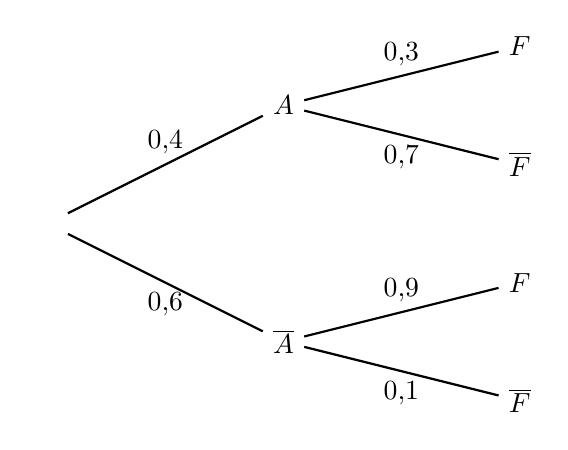
\begin{tikzpicture}[thick, scale=1.5]
\node (P_-1_0) at (-2,-1.5) {$\phantom{A}$};
\node (P_0_0) at (0,-0.5) {$A$};
\draw (P_-1_0) -- (P_0_0) node[midway, above] {$0{,}4$};
\node (P_1_0) at (2,-0) {$F$};
\draw (P_0_0) -- (P_1_0) node[midway, above] {$0{,}3$};
\node (P_1_1) at (2,-1) {$\overline{F}$};
\draw (P_0_0) -- (P_1_1) node[midway, below] {$0{,}7$};
\node (P_0_2) at (0,-2.5) {$\overline{A}$};
\draw (P_-1_0) -- (P_0_2) node[midway, below] {$0{,}6$};
\node (P_1_2) at (2,-2) {$F$};
\draw (P_0_2) -- (P_1_2) node[midway, above] {$0{,}9$};
\node (P_1_3) at (2,-3) {$\overline{F}$};
\draw (P_0_2) -- (P_1_3) node[midway, below] {$0{,}1$};
\end{tikzpicture}
\end{center}

\subsection*{2.}

On calcule : \(p(A \cap \overline{F}) = p(A) \times p_A(\overline{F}) = 0{,}4 \times 0{,}7 = 0{,}28\).

\subsection*{3.}

On a aussi :
\[
p(\overline{A} \cap \overline{F}) = p(\overline{A}) \times p_{\overline{A}}(\overline{F}) = 0{,}6 \times 0{,}1 = 0{,}06.
\]
Or, d'après la loi des probabilités totales :
\[
p(\overline{F}) = p(A \cap \overline{F}) + p(\overline{A} \cap \overline{F}) = 0{,}28 + 0{,}06 = 0{,}34.
\]

\subsection*{4.}

Il faut trouver :
\[
p_{\overline{F}}(A) = \dfrac{p(A \cap \overline{F})}{p(\overline{F})} = \dfrac{0{,}28}{0{,}34} \approx 0{,}8235 \approx 0{,}82.
\]

\subsection*{5.}

On a vu que la probabilité de choisir un participant ayant choisi un séjour à l'étranger est égale à \(0{,}34\).

Donc la probabilité d'interroger deux participants (avec éventuellement deux fois le même participant) ayant choisi un séjour à l'étranger est égale à : \(0{,}34 \times 0{,}34 = 0{,}1296\).

Donc la probabilité qu'au moins un des deux participants ait choisi un séjour en France est égale à : \(1 - 0{,}1296 = 0{,}8704 \approx 0{,}87\).

